\documentclass[12pt]{article}

\usepackage[dvips]{graphicx}
\graphicspath{{images/}}
\usepackage{/home/z/mydefines}

\geometry{
    a4paper,
    left=1cm, top=1.5cm,
    right=1cm, bottom=2cm
}

\usepackage{enumitem}
\usepackage{fancyhdr}
\setlength{\headheight}{15.6pt}
\pagestyle{fancy}
\fancyfoot{}
\lhead{Август 2017 \hfill Алые Паруса \hfill 7-8 класс}
\begin{document}

\centerline{\Large \bf Игра}
{\bf Правила игры}. Вы колонизируете территорию. Изначально вам доступен кусок земли. За захват
новых территорий вы платите задачами. За базовый захват вы платите 1 задачу + (1 задачу, если
территория принадлежит другой команде) + (1 задачу, если захватываемая территория не граничит с
вашей).

Захват происходит следующим образом: вы пишете на небольшом листке
\begin{itemize}
\item номер команды
\item захватываемая территория
\item № 1-й задачи - ответ
\item № 2-й задачи - ответ
\\
\ldots
\end{itemize}
Нужно сдавать столько задач, сколько вам нужно для захвата. Если задач не хватает, или к хотя бы одной
задаче ответ неправильный, то вам начисляется одно штрафное очко, и захват не происходит. Иначе
захват происходит успешно, и территория переходит к вам. В каждой задаче, где ответ можно
представить в виде числа, его нужно представить в виде числа.
\hr

\centerline{\large \bf Подсчёт очков}

В конце игры подсчитывается количество удерживаемых на этот момент территорий, а также количество
штрафных очков. Команды сортируются по убыванию количества территорий, а при равенстве -- по
возрастанию количества штрафов.
\hr

\centerline{\large \bf Условия Задач}
\begin{enumerate}
\item Найдите остаток от деления -4251 на 59.
\item В графе 14 вершин степени 3, 6 вершин степени 4, всего 45 ребер. Сколько всего вершин, если
остались только вершины степени 2?
\item сколько различных слов, не обязательно осмысленных, можно составить переставляя буквы в слове
КОЛОКОЛ?

\begin{minipage}{0.5\textwidth}
\item Сколько способов для черепахи добраться из левого ряда в правый, если за один ход она
перемещается так, как показано на рисунке?
\item Упростите выражение. Представьте ответ в виде $a \cdot 2^{b}$
\[ \frac{2 \cdot 2^{2n + 1} - 2^{2n} + 4^{n + 1}}{2}\]
\item Найдите корни уравнения
\[ 2x^2 - 4x + 7 = x^2 - 6x + 70\]
\end{minipage}
\begin{minipage}{0.4\textwidth}
\rightline{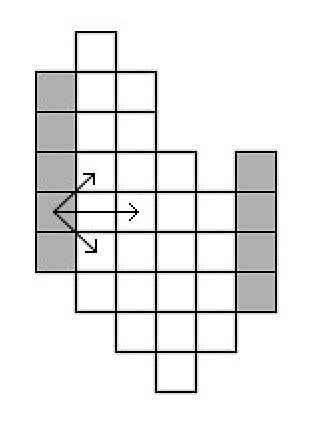
\includegraphics[width=0.5\linewidth]{img1.eps}}
\end{minipage}
\item Найдите (какое-нибудь) решение в целых числах уравнения
\[ 21x + 57y = \text{НОД}(21, 57)\]
\item Забор из 11 досок красят в 3 цвета. Сколько существует способов покраски, если красить
соседние доски в разные цвета.
\item Дан граф из 17 вершин. Максимальное кол-во комнонент связности при 42 ребрах и минимальное при
12 ребрах (2 ответа).
\item Из трех неравенств $x^2 - x > 0, 4x < 10$ и $10x > 62$ ровно 1 истинно. Найдите все целые $x$.
\item В правильном треугольнике $ABC$ проведена высота $AH$. В треугольнике $AHC$ проведена высота $HM$.
Найти $MC$, если $AB = 8$.
\item Разрежьте квадрат на четыре части так, чтобы каждая часть соприкасалась (т.е. имела общие
участки границы) с тремя другими.
\item Куб с ребром длиной 5 м разрезан на кубики, ребро каждого из которых равно 2 см. Эти кубики
выложили в один сплошной ряд. Чему равна длина этого ряда? (в метрах)
\item Даны 11 чисел. Какое наибольшее количество попарных сумм этих чисел может быть нечётными
числами?
\item Пять первоклассников стояли в шеренгу и держали 37 флажков. У всех школьников, стоящих справа
от Тани — 14 флажков, справа от Яши — 32, справа от Веры — 20, справа от Максима — 8. Сколько
флажков у Даши?
\item Дана трапеция $ABCD$ с основаниями $AD = 7$ и $BC = 2$. $\angle A = 60^{\circ}, \angle D =
30^{\circ}$. Найти длину отрезка, соединяющего середины оснований.
\item Учитель записал Пете в тетрадь четыре различных натуральных числа. Для каждой пары этих
чисел Петя нашёл их наибольший общий делитель. У него получились шесть чисел: $1, 2, 3, 4, 5$ и $N$, где
$N > 5$. Какое наименьшее значение может иметь число $N$?
\item Напишите 5 любых решений в натуральных числах уравнения $a^2 + b^2 = c^2$, где НОД$(a,b,c)=1$
\item Найдите НОД чисел 111…11 (100 единиц) и 11..11 (60 единиц).
\item Сколько натуральных чисел, меньших тысячи, не делятся ни на 5, ни на 7?
\item Сколькими способами можно выбрать из 36 карт 4 карты так, чтобы среди выбранных
был хотя бы один туз?
\end{enumerate}
\end{document}
